% --------------------------------------------------------------
% This is all preamble stuff that you don't have to worry about.
% Head down to where it says "Start here"
% --------------------------------------------------------------
 
\documentclass[12pt]{article}
 
\usepackage[margin=1in]{geometry} 
\usepackage{amsmath,amsthm,amssymb}
\usepackage{xcolor}
\usepackage{listings}
\usepackage{graphicx}
\usepackage{hyperref}
\usepackage{listings}
\usepackage{stackengine}
\usepackage{array}
\graphicspath{{/home/arpit/Desktop/iitd/sem_7/COL334/projects/Getting-To-Know-Network-Traffic/img}}

\newcommand{\N}{\mathbb{N}}
\newcommand{\Z}{\mathbb{Z}}
 
\newenvironment{theorem}[2][Theorem]{\begin{trivlist}
\item[\hskip \labelsep {\bfseries #1}\hskip \labelsep {\bfseries #2.}]}{\end{trivlist}}
\newenvironment{lemma}[2][Lemma]{\begin{trivlist}
\item[\hskip \labelsep {\bfseries #1}\hskip \labelsep {\bfseries #2.}]}{\end{trivlist}}
\newenvironment{exercise}[2][Exercise]{\begin{trivlist}
\item[\hskip \labelsep {\bfseries #1}\hskip \labelsep {\bfseries #2.}]}{\end{trivlist}}
\newenvironment{problem}[2][Problem]{\begin{trivlist}
\item[\hskip \labelsep {\bfseries #1}\hskip \labelsep {\bfseries #2.}]}{\end{trivlist}}
\newenvironment{question}[2][Question]{\begin{trivlist}
\item[\hskip \labelsep {\bfseries #1}\hskip \labelsep {\bfseries #2.}]}{\end{trivlist}}
\newenvironment{corollary}[2][Corollary]{\begin{trivlist}
\item[\hskip \labelsep {\bfseries #1}\hskip \labelsep {\bfseries #2.}]}{\end{trivlist}}

\newenvironment{solution}{\begin{proof}[Solution]}{\end{proof}}
\definecolor{codegreen}{rgb}{0,0.6,0}
\definecolor{codegray}{rgb}{0.5,0.5,0.5}
\definecolor{codepurple}{rgb}{0.58,0,0.82}
\definecolor{backcolour}{rgb}{0.95,0.95,0.92}

\lstdefinestyle{mystyle}{
    backgroundcolor=\color{backcolour},   
    commentstyle=\color{codegreen},
    keywordstyle=\color{magenta},
    numberstyle=\tiny\color{codegray},
    stringstyle=\color{codepurple},
    basicstyle=\ttfamily\footnotesize,
    breakatwhitespace=false,         
    breaklines=true,                 
    captionpos=b,                    
    keepspaces=true,                 
    numbers=left,                    
    numbersep=5pt,                  
    showspaces=false,                
    showstringspaces=false,
    showtabs=false,                  
    tabsize=2
}
\lstset{style=mystyle}
\begin{document}
 
% --------------------------------------------------------------
%                         Start here
% --------------------------------------------------------------
 
\title{Assignment 2: Socket Programming}
\author{Arpit Prasad and Akshat Bhasin\\ 
COL334: Computer Network}

\maketitle
\section{Part 1: Word Counting Client}

\begin{figure}[h!]
    \centering
    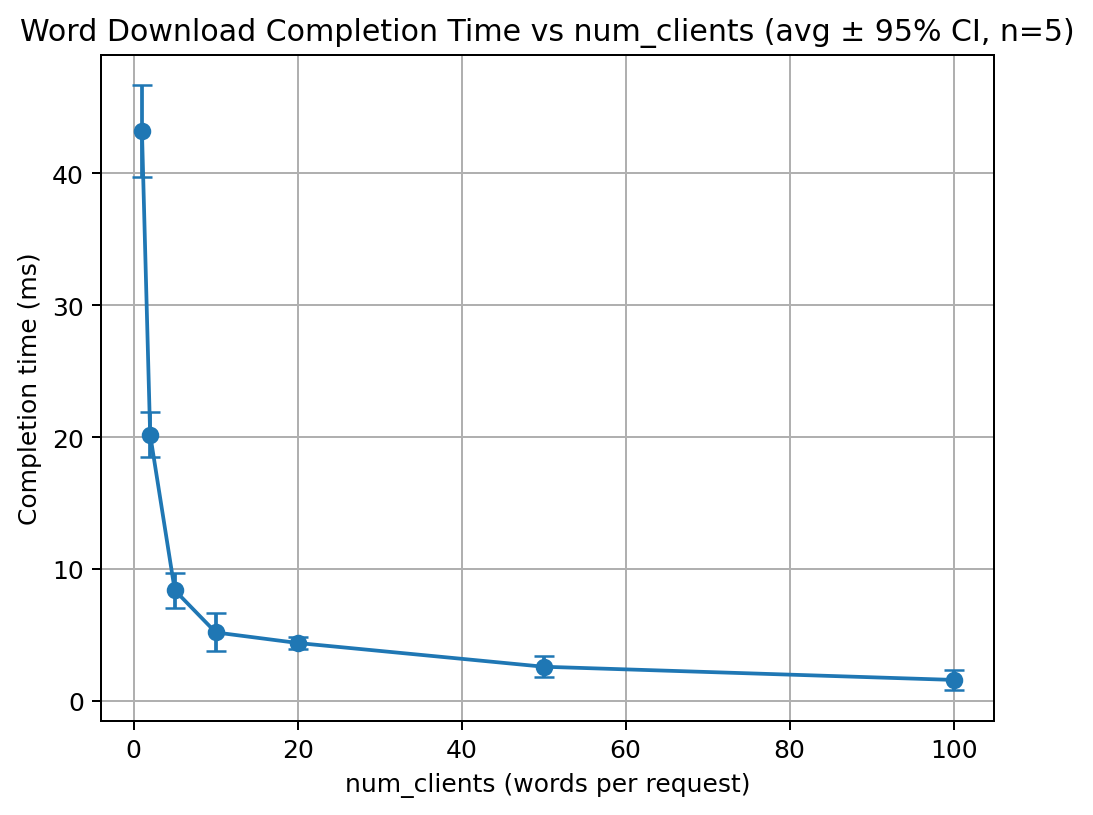
\includegraphics[width=0.8\textwidth]{/home/arpit/Desktop/iitd/sem_7/COL334/projects/Socket-Programming/part1/p1_plot.png}
    \caption{Completion Time vs Varying Size of chunks for file download}
    \label{fig:part1_output}
\end{figure}

\subsection{Implementation Details}
\begin{enumerate}
    \item \textbf{Client-Server Model}: The implementation follows a client-server architecture where the server listens for incoming connections and the client requests file downloads.
    \item \textbf{Client Requests}: The client sends a request to the server specifying the file to be downloaded and the chunk size. The client downloads the entire file by continuously varying the offset and requesting chunks of the specified size until the entire file is received.
    \item \textbf{Server Response}: The server reads the requested file in chunks of the specified size and sends each chunk back to the client.
\end{enumerate}

\subsection{Observations}
\begin{enumerate}
    \item \textbf{Trend in Graph}
    \begin{enumerate}
        \item \textbf{Decay}: As the chunk size increases, the completion time decreases. 
        \item \textbf{Reason}: This is because larger chunks reduce the overhead of multiple read and write operations, leading to more efficient data transfer.
    \end{enumerate}
    \item \textbf{Trend in Variance}
    \begin{enumerate}
        \item \textbf{Decay in Variance}: The variance in completion time also decreases with increasing chunk size.
        \item \textbf{Reason}: This is because larger chunks lead to more consistent transfer times, reducing the impact of network fluctuations and other transient factors.
    \end{enumerate}
    \item \textbf{Optimal Chunk Size}
    \begin{enumerate}
        \item \textbf{Optimal Chunk Size}: There is a point of diminishing returns where increasing the chunk size further does not significantly reduce the completion time.
        \item \textbf{Reason}: This is due to factors such as network latency and server processing time becoming the dominant contributors to total transfer time.
    \end{enumerate}
    
\end{enumerate}

\section{Part 2: Concurrent Word Counting Server}

\subsection{Implementation Details}
\begin{enumerate}
    \item \textbf{Concurrency Model}: The server uses a multi-threaded approach to handle multiple client requests simultaneously. Each client connection is handled in a separate thread.
    \item \textbf{Client Requests}: Clients send a request to the server specifying the file to be processed and the chunk size. The client reads the entire file in chunks of the specified size and sends each chunk to the server for word counting.
    \item \textbf{Server Response}: The server processes each chunk received from the client, counts the words, and sends the count back to the client.
\end{enumerate}

\subsection{Observations}

\begin{figure}[h!]
    \centering
    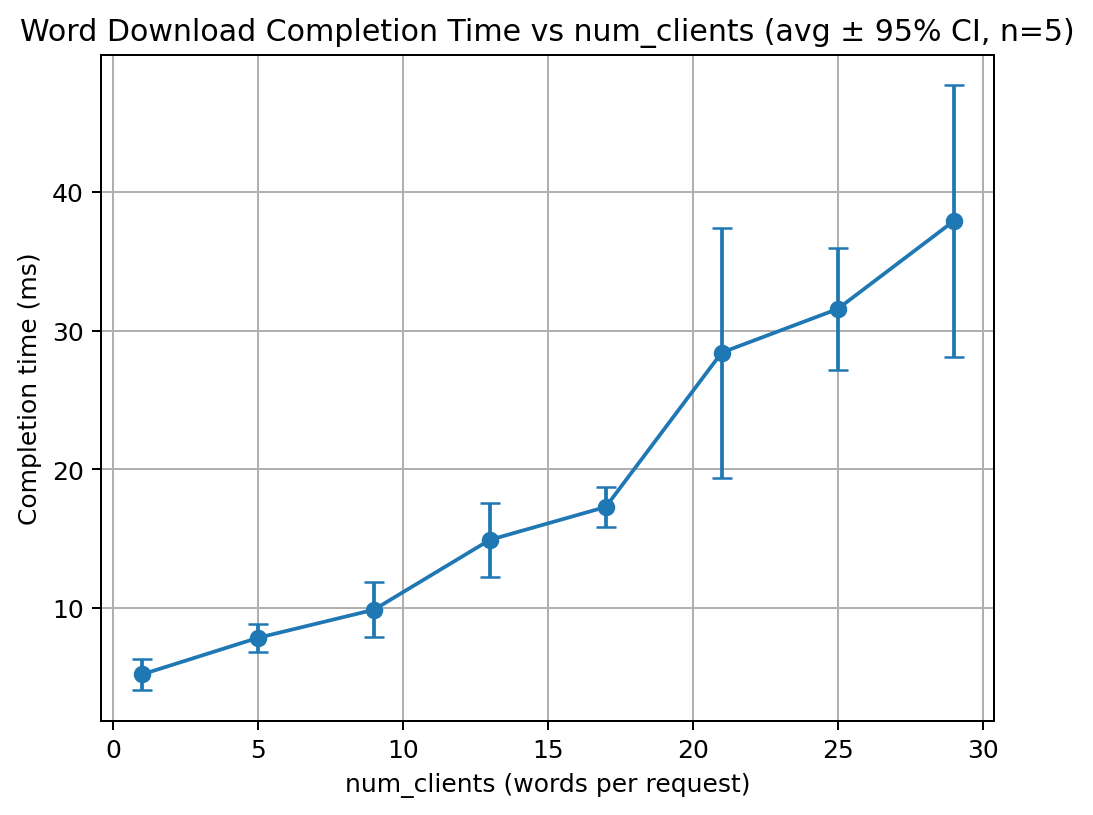
\includegraphics[width=0.8\textwidth]{/home/arpit/Desktop/iitd/sem_7/COL334/projects/Socket-Programming/part2/p2_plot.png}
    \caption{Average Completion Time vs Varying Number of Clients}
    \label{fig:part2_output}
\end{figure}

\begin{enumerate}
    \item \textbf{Trend in Graph}
    \begin{enumerate}
        \item \textbf{Increase}: As the number of clients increases, the average completion time also increases.
        \item \textbf{Reason}: This is because the server has to handle more requests simultaneously, leading to increased contention for server resources.
    \end{enumerate}
    \item \textbf{Trend in Variance}
    \begin{enumerate}
        \item \textbf{Increase in Variance}: The variance in completion time also increases with the number of clients.
        \item \textbf{Reason}: This is due to the increased contention for server resources, leading to more variability in processing times.
    \end{enumerate}
    \item \textbf{Scalability}
    \begin{enumerate}
        \item \textbf{Scalability Limitations}: There is a point where adding more clients leads to a significant increase in completion time.
        \item \textbf{Reason}: This is due to the server reaching its maximum capacity for handling concurrent connections, leading to increased queuing delays.
    \end{enumerate}
\end{enumerate}

\section{Part 3: When Client Gets Greedy}

\subsection{Implementation Details}
\begin{enumerate}
    \item \textbf{Client Behavior}: One of the clients sends multiple requests to the server in back to back without waiting for the server to respond to previous requests.
    \item \textbf{Server Handling}: The server processes each request as it arrives, but the rapid back to back requests can lead to increased wait times for other clients to utilise the servers resources.
\end{enumerate}

\subsection{Observations}

\begin{figure}[h!]
    \centering
    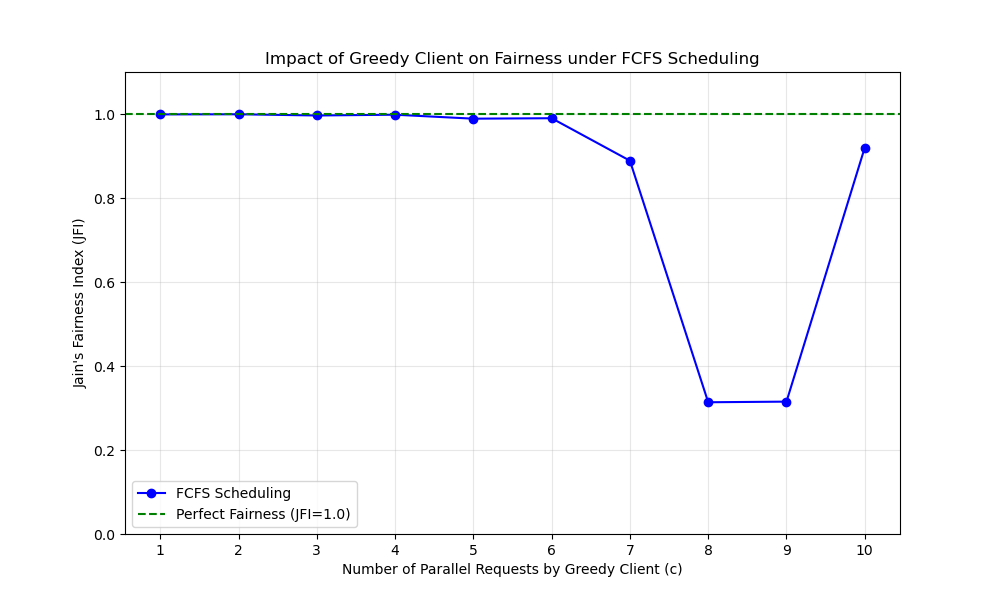
\includegraphics[width=0.8\textwidth]{/home/arpit/Desktop/iitd/sem_7/COL334/projects/Socket-Programming/part3/p3_plot.png}
    \caption{Jain's Fairness Index vs Number of back to back requests by a single client in a system of 10 Clients}
    \label{fig:part3_output}
\end{figure}

\begin{enumerate}
    \item \textbf{Trend in Graph}
    \begin{enumerate}
        \item \textbf{Decrease}: As the number of back to back requests by a single client increases, the Jain's Fairness Index decreases. However here the decrease is not very significant, in fact the handling of server seem almost fair.
        \item \textbf{Reason}: Ideally, the fairness index should decrease as one client monopolizes server resources, leading to increased wait times for other clients. However, for small number of back to back requests, the server can still manage to handle requests from other clients in a timely manner, leading to a relatively high fairness index.
    \end{enumerate}
    \item \textbf{Aymptotic Behaviour of Jain's Fairness Index}
    \begin{enumerate}
        \item \textbf{For larger c values}: For larger number of back to back requests, the fairness index would decrease more significantly as the greedy client would dominate server resources, leading to increased wait times for other clients. For $c = 100$ we obtained a JFI score of 0.25.
        \item \textbf{Reason}: From the formula of JFI, if we take the limit of one client getting all the resources and others getting none, the JFI would tend to $1/n_{clients}$, where $n_{clients}$ is the number of clients in the topology. This is because both the numerator and denominator would be dominated by the resources allocated to the greedy client.
    \end{enumerate}     
    \item \textbf{Impact on Other Clients}
    \begin{enumerate}
        \item \textbf{Increased Wait Times}: Other clients experience increased wait times as the greedy client monopolizes server resources.
        \item \textbf{Reason}: The server has to process multiple requests from the greedy client before it can attend to requests from other clients, leading to increased wait times.
    \end{enumerate}
\end{enumerate}

\section{Part 4: When the Server Enforces Fairness}

\subsection{Implementation Details}
\begin{enumerate}
    \item \textbf{Server Behavior}: The server implements a fairness mechanism to ensure that no single client can monopolize server resources. This is achieved by round-robin scheduling of client requests.
    \item \textbf{Client Requests}: Clients send requests to the server specifying the file to be processed and the chunk size. The client reads the entire file in chunks of the specified size and sends each chunk to the server for word counting.
    \item \textbf{Server Response}: The server processes each chunk received from the clients in a round-robin manner, counts the words, and sends the count back to the respective client.
\end{enumerate}

\subsection{Observations}

\begin{figure}[h!]
    \centering
    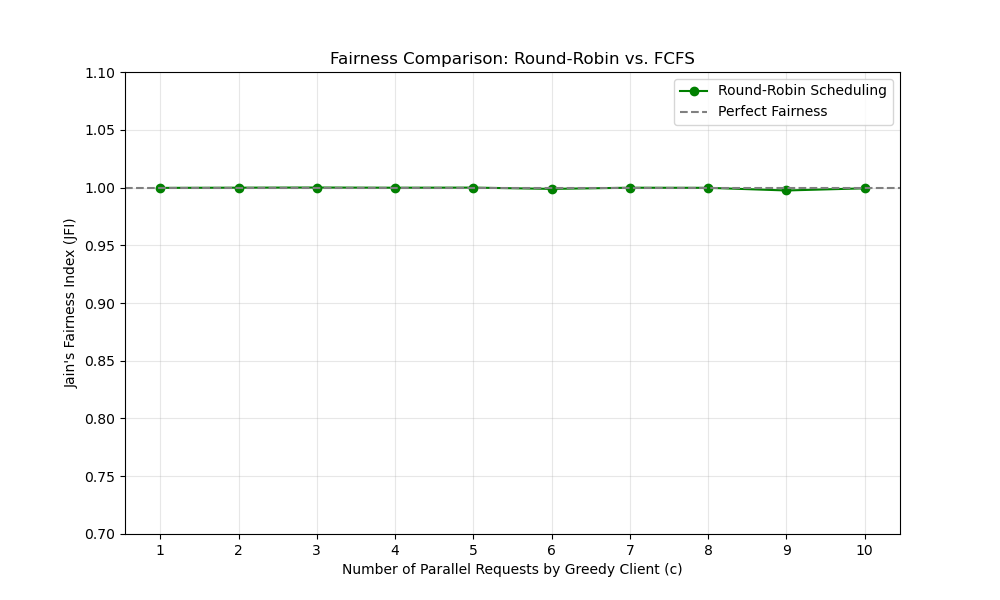
\includegraphics[width=0.8\textwidth]{/home/arpit/Desktop/iitd/sem_7/COL334/projects/Socket-Programming/part4/p4_plot.png}
    \caption{Jain's Fairness Index vs Number of back to back requests by a single client in a system of 10 Clients with server enforcing fairness with round robin scheduling}
    \label{fig:part4_output}
\end{figure}

\begin{enumerate}
    \item \textbf{Trend in Graph}
    \begin{enumerate}
        \item \textbf{Stable JFI}: As the number of back to back requests by a single client increases, the Jain's Fairness Index remains relatively stable and high.
        \item \textbf{Reason}: The round-robin scheduling ensures that each client gets a fair share of server resources, preventing any single client from monopolizing the server.
        \item Slight decrease in JFI: There is a slight decrease in JFI as the number of back to back requests increases, but it is not significant.
        \item Reason: This is because even with round-robin scheduling, a client sending a large number of back to back requests can still lead to increased wait times for other clients, but the impact is mitigated by the fairness mechanism. (Explained in Limitations of Round Robin Scheduling)
    \end{enumerate}
    \item \textbf{Impact on Other Clients}
    \begin{enumerate}
        \item \textbf{Reduced Wait Times}: Other clients experience reduced wait times as the server enforces fairness.
        \item \textbf{Reason}: The round-robin scheduling ensures that the server attends to requests from all clients in a timely manner, reducing wait times.
    \end{enumerate}
    \item \textbf{Effectiveness of Fairness Mechanism}
    \begin{enumerate}
        \item \textbf{High JFI}: The Jain's Fairness Index remains high even with increasing back to back requests from a single client.
        \item \textbf{Reason}: This indicates that the fairness mechanism is effective in ensuring equitable resource allocation among clients.
    \end{enumerate}
    \item \textbf{Limitations of Round Robin Scheduling}
    \begin{enumerate}
        \item How can client still monopolize server resources: If a client sends a very large number of back to back requests, it can still lead to increased wait times for other clients, even with round-robin scheduling.
        \item Reason: This is because the server has to process each request in turn, and a large number of requests from one client can lead to increased overall processing time, affecting the responsiveness for other clients.
    \end{enumerate}
\end{enumerate}

% --------------------------------------------------------------
%     You don't have to mess with anything below this line.
% --------------------------------------------------------------

\end{document}
